\documentclass[11pt]{article}
\usepackage[margin=1.25in]{geometry}    % Better margins for readability
\usepackage{graphicx}
\usepackage{setspace} % For line spacing
\usepackage{hyperref}
\usepackage[T1]{fontenc}                % Better character support
\usepackage[utf8]{inputenc}             % Input encoding
\usepackage[default]{FiraSans}          % Highly readable font [6]
\usepackage{caption}                   % For better figure captions

\title{LIS 470 -- Assignment A5 \\
Brainstorming}
\author{Team 5 \\
Alejandro De La Torre \\
Angelique Carrillo \\
Helena Huang \\
Yanbin Chen \\
Peixin Yang}
\date{Spring 2026}

\begin{document}

\maketitle

\vspace{1cm}

\section*{How Might We Prompt}

How might we simplify grocery shopping for college students so that they can quickly find affordable food, plan meals, and stay within budget?

\vspace{0.5cm}

\section*{Brainstorming Session}

During our studio session, our team worked together to generate as many ideas as possible related to our design problem. We began by writing our “How might we” statement at the top of the board so that it remained visible throughout the brainstorming process. This helped us stay focused on the goal of helping college students shop for groceries more efficiently and affordably.

We started by individually writing down ideas and then building on each other’s contributions. As we continued brainstorming, new ideas emerged naturally from conversations and reactions to earlier suggestions. Some ideas focused on saving money, while others focused on improving organization, collaboration with roommates, or helping students navigate grocery stores more easily.

As the board filled up, we began grouping similar ideas together. Several themes emerged during this process, including \textbf{Price}, \textbf{Collaboration}, \textbf{Meal Planning}, and \textbf{Store Frustrations}. Organizing the ideas into these categories helped us better understand the types of problems students face while grocery shopping.

Once our ideas were grouped, we used dot voting to identify which concepts we thought had the most potential. Each team member placed dots on the ideas they were most interested in exploring further. The ideas that received the most support became the ones we chose to develop further as a team.

\vspace{0.5cm}

\begin{center}
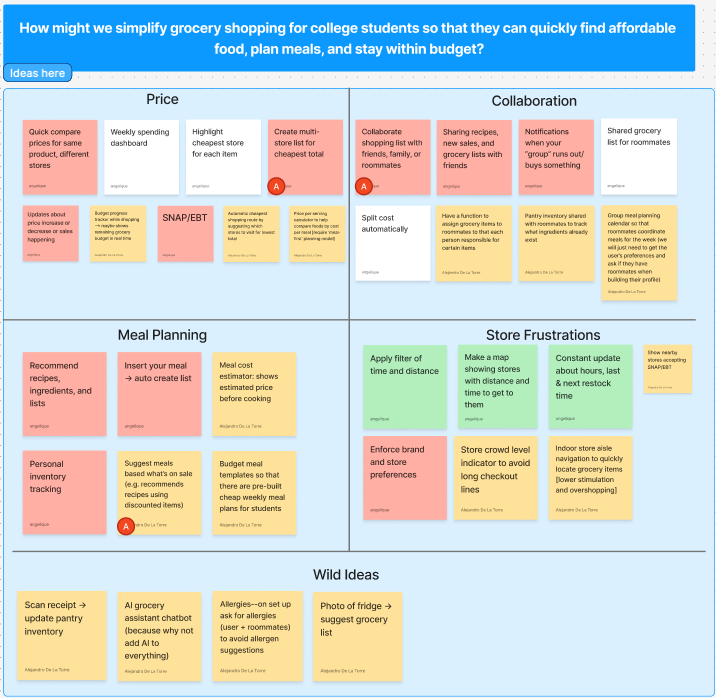
\includegraphics[width=\textwidth]{../boards/board_v3.png}
\captionof{figure}{\textit{Brainstorming board showing grouped ideas and dot voting results.}}
\end{center}

\vspace{0.5cm}

\section*{Selected Ideas for Further Development}

After reviewing the results of our brainstorming and discussing the ideas that received the most interest during dot voting, we selected three concepts that we believe best address our design challenge.

\subsection*{1. Smart Grocery Price Comparison Tool}

One of the strongest themes that emerged during our brainstorming session was the difficulty students face when trying to find affordable groceries. Many of our ideas focused on comparing prices between stores or helping students stay within a grocery budget.

This concept focuses on a tool that allows students to quickly compare prices for grocery items across different stores. A user could enter a shopping list and the system would highlight the cheapest store for each item or suggest the most affordable overall shopping plan. The tool could also notify users about sales, price changes, or discounts. By making price information more transparent, this system would help students make more informed purchasing decisions.

\subsection*{2. Collaborative Grocery Lists for Roommates}

Another major theme from our brainstorming session was collaboration. Many college students live with roommates and share responsibilities when it comes to grocery shopping.

This idea involves a shared grocery list system that allows multiple users to contribute to the same list. Roommates could add items, track what has already been purchased, and automatically split the cost of shared groceries. The system could also send notifications when common household items are running low. This would help reduce confusion and make it easier for groups of students to coordinate grocery shopping.

\subsection*{3. Budget-Friendly Meal Planning Assistant}

Several of our ideas also focused on helping students plan meals more effectively. Many students struggle to balance cost, time, and convenience when deciding what to cook.

This concept centers around a meal planning assistant that recommends recipes based on a student’s budget and available ingredients. The system could generate grocery lists automatically, suggest meals based on current grocery store sales, and estimate the cost of meals before cooking. By connecting meal planning with budgeting tools, this idea could help students save money while still eating balanced meals.

\section*{Reflection}

Overall, our brainstorming session was productive and engaging. One thing that went well was the variety of ideas we were able to generate in a relatively short period of time. Because everyone approached the problem from a slightly different perspective, our ideas covered a wide range of possibilities, including budgeting tools, collaborative grocery systems, meal planning assistants, and even more experimental concepts like AI grocery helpers.

Another positive aspect of the session was how we built on each other’s ideas. Many concepts started as simple suggestions and gradually evolved as other team members added new features or improvements. This collaborative process helped us develop more interesting and well-rounded ideas.

One challenge we encountered was deciding which ideas to prioritize. Since many of our ideas addressed different aspects of the grocery shopping experience, it was not always easy to compare them directly. Using dot voting helped us resolve this by visually identifying the ideas that received the most interest from the group.

If we were to repeat this process in the future, we would likely spend more time creating quick sketches or visual representations of our ideas. While the post-it notes helped capture the basic concepts, adding small sketches might help communicate ideas more clearly and spark additional creativity.

\end{document}